% =====================================================================
\chapter{Eredmények}
\label{ch:eredmenyek}
% =====================================================================

Ebben a fejezetben a pilot vizsgálat eredményeit közöljük. A pilot célja nem a hipotézisek
eldöntése volt -- egyetlen dokumentumon ez \az{\ref{sec:statisztika}}.~szakasz szerint elvileg sem
lehetséges --, hanem (i) a teljes mérési lánc validálása, (ii) a komponensek hatásának és költségének
előzetes becslése, és (iii) a fő vizsgálat tervének megalapozása. Minden közölt szám a
\code{tests/eval/results\_pilot} könyvtár nyers adataiból, a keretrendszer \code{report} lépésével
készült; a táblázatok és a nyers adatok közötti megfeleltetést \az{\ref{app-reprodukcio}}.~függelék adja meg.

\section{A pilot beállításai}

A pilot a \code{hu-coffee} dokumentumon futott: egy 1\,702 karakteres magyar oktatási szöveg a kávé
eredetéről, fajtáiról, termesztéséről és feldolgozásáról, könnyű vizsgaszinttel. A szemantikus darabolás
négy darabot adott (a szórásalapú és a rögzített darabolás hármat). Minden kar dokumentumonként három
vizsgát generált (magok: 1, 2, 3), vizsgánként tíz feleletválasztós kérdéssel, így karonként 30,
összesen 300 kérdés készült. A tíz kar: \arm{E0}, \arm{E1}, \arm{E2}, \arm{E2f}, \arm{E2h}, \arm{E3},
\arm{E4}, \arm{E5a}, \arm{E5b}, \arm{E5c}; az \arm{E4b} kar futása nem fejeződött be, és a teljes
dokumentumos alapvonalak, valamint az \arm{E2x} kar a pilot után készültek el.

A helyi karok egy asztali PC fogyasztói GPU-ján (NVIDIA GeForce RTX 3070 Ti, 8\,GB) futottak, a
generátor 16\,384 tokenes kontextussal. A pilot még \az{\ref{ch:modszer}}.~fejezetben „új”-ként jelölt
szabályok nélkül futott: a tervezett karokban $r=2$ újrapróbálkozás volt engedélyezve, szivárgási
szabályok és javító hívás nélkül. A bíró a teljes dokumentumot látta (\code{judge-v1}), ami egy
ilyen rövid szövegnél lényegében azonos a kérdés kontextusával.

\section{Összesített eredmények}

\Az{\ref{tab:pilot-fo}}.~táblázat a karonkénti fő mutatókat a minőségi index szerint csoportosítva mutatja.
\Az{\ref{fig:mutatok}}.~ábra ugyanezeket a mutatókat hőtérképként, a visszakeresési találati aránnyal
kiegészítve ábrázolja.

\begin{table}[htbp]
\centering
\caption{A pilot fő eredményei: egy magyar dokumentum, 3 mag, karonként 30 kérdés. Ráták
\%-ban. $Q$: minőségi index; Form.: formai megfelelés; Alát.: alátámasztottság; Vak: vak megoldhatóság;
Diszt.: disztraktor-validitás; Lef.: lefedettség; Sziv.: kulcs a törzsben; Nell.: nem ellenőrzött kérdések
száma vizsgánként; Hívás: átlagos modellhívás vizsgánként; Perc: medián futási idő vizsgánként.}
\label{tab:pilot-fo}
\small
\setlength{\tabcolsep}{4pt}
\begin{tabular}{@{}lcccccccccr@{}}
\toprule
Kar & $Q$ & Form. & Alát. & Vak & Diszt. & Lef. & Sziv. & Nell. & Hívás & Perc \\
\midrule
\arm{E0}  & 0,83 & 100 & 67 & 85 & 80 & 50 & 0 & -- & 1 & 0,3 \\
\arm{E1}  & 0,88 & 100 & 73 & 93 & 87 & 58 & 0 & 2,0 & 23 & 3,0 \\
\arm{E2}  & 0,76 & 67 & 73 & 77 & 89 & 58 & 3 & 4,3 & 75 & 6,2 \\
\arm{E2f} & 0,73 & 67 & 53 & 82 & 90 & 58 & 7 & 3,3 & 59 & 5,3 \\
\arm{E2h} & 0,76 & 67 & 67 & 79 & 93 & 67 & 10 & 4,0 & 76 & 6,7 \\
\arm{E3}  & 0,85 & 67 & 87 & 100 & 87 & 50 & 20 & 6,0 & 101 & 8,0 \\
\midrule
\arm{E4}  & \textbf{0,99} & 100 & 100 & 100 & 97 & \textbf{25} & 0 & -- & 1 & 6,6 \\
\midrule
\arm{E5a} & 0,90 & 100 & 80 & 86 & 93 & 50 & 0 & -- & 1 & 0,3 \\
\arm{E5b} & 0,90 & 100 & 80 & 90 & 91 & 56 & 0 & -- & 1 & 0,3 \\
\arm{E5c} & 0,81 & 100 & 60 & 79 & 83 & 67 & 0 & -- & 1 & 0,3 \\
\bottomrule
\end{tabular}
\end{table}


\begin{figure}[htbp]
\centering
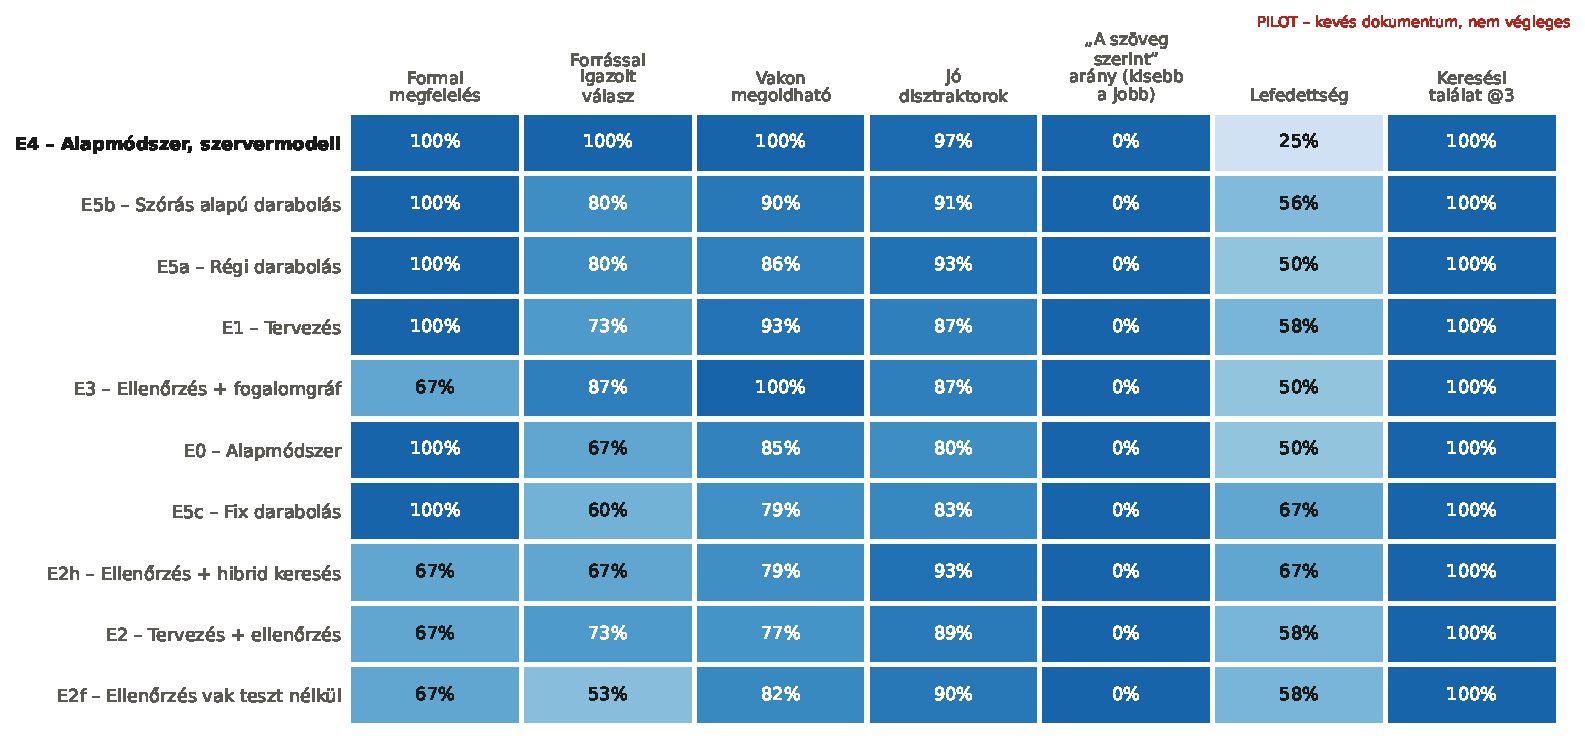
\includegraphics[width=\textwidth]{figures/abra3_mutatok.pdf}
\caption{Az egyes minőségi mutatók karonként (pilot). A „szöveg szerint” oszlop a meta-hivatkozások
aránya, a keresési találat@3 a referenciakérdések bizonyító mondatának visszakeresési aránya.}
\label{fig:mutatok}
\end{figure}

Három megfigyelés emelhető ki. \emph{Először}, a helyi karok minőségi indexe 0,73 és 0,90 között
szóródik, a szervermodell (\arm{E4}) pedig 0,99-cel kiemelkedik. \emph{Másodszor}, a tervezés
(\arm{E1}) a naiv alapvonalhoz képest minden tartalmi mutatón javított, az ellenőrző karok
(\arm{E2}, \arm{E2f}, \arm{E2h}, \arm{E3}) viszont a formai megfelelésben 67\,\%-ra estek vissza, ami a
$Q$ indexüket jelentősen lerontotta. \emph{Harmadszor}, a lefedettség a szervermodellnél a
legalacsonyabb (25\,\%): a legjobb minőségű kar a dokumentum négy darabjából egyre koncentrált. A
visszakeresési találati arány minden karon 100\,\% volt, ami egy négydarabos dokumentumon várható
(a három visszakeresett darab a négyből szinte mindig tartalmazza a bizonyítékot); a visszakeresés
mutatói csak a hosszú dokumentumokon lesznek informatívak.

\section{A tervezés hatása (RQ1, RQ2)}

A naiv alapvonal (\arm{E0}) és a tervezett, de nem ellenőrzött csővezeték (\arm{E1}) összevetése
(\ref{tab:pilot-fo}. és \ref{tab:rubrika-eredmeny}.~táblázat) szerint a tervezés azonos modell és azonos formai megfelelés mellett javította az alátámasztottságot
($+6$ százalékpont), a vak megoldhatóságot ($+8$), a disztraktor-validitást ($+7$) és a lefedettséget
($+8$), a bíró helyességi pontszámát 3,5-ről 3,7-re, disztraktorpontszámát 3,5-ről 4,0-ra, a
„felhasználnám” arányt 63-ról 67\,\%-ra emelte, az érthetőségi pontszám viszont 4,7-ről 4,0-ra csökkent. Az ára: 23-szoros hívásszám és
9-szeres futási idő (20 másodperc helyett 3 perc).


Az érthetőség csökkenése mögött a kérdések formájának megváltozása áll: az egyenkénti generálás
hosszabb törzseket és jóval hosszabb válaszlehetőségeket eredményezett (\ref{tab:hosszak}.~táblázat).
A naiv alapvonal egy vizsgán belül rövid, tényfelidéző kérdéseket írt, 60 karakteres átlagos
törzzsel és négy opcióra összesen 60 karakterrel („9. század”, „10. század”, \dots); a tervezett
csővezeték kérdései átlagosan 88 karakteres törzsűek, az opciók együttes hossza pedig 315 karakter,
vagyis tipikusan teljes mondatok. Ez a fogalmi, magyarázó kérdéseknek kedvez (a disztraktorpontszám
nőtt), de a kérdés olvasási terhét is növeli.

\begin{table}[htbp]
\centering
\caption{A kérdések hossza, változatossága és tematikus hasonlósága karonként (pilot, átlagok 30
kérdésen). Törzs: a törzs karakterszáma; Opciók: a négy opció együttes karakterszáma; Dup.: duplikátumráta;
RefSim: átlagos maximális hasonlóság a referenciakérdésekhez.}
\label{tab:hosszak}
\small
\begin{tabular}{@{}lrrcc@{}}
\toprule
Kar & Törzs & Opciók & Dup. (\%) & RefSim \\
\midrule
\arm{E0}  & 60  & 60  & 16 & 0,895 \\
\arm{E1}  & 88  & 315 & 21 & 0,912 \\
\arm{E2}  & 84  & 348 & 21 & 0,909 \\
\arm{E2f} & 95  & 405 & 17 & 0,911 \\
\arm{E2h} & 93  & 352 & 14 & 0,907 \\
\arm{E3}  & 120 & 365 & 25 & 0,895 \\
\arm{E4}  & 54  & 87  & 4  & 0,890 \\
\arm{E5a} & 65  & 88  & 16 & 0,898 \\
\arm{E5b} & 58  & 73  & 10 & 0,891 \\
\arm{E5c} & 57  & 36  & 45 & 0,885 \\
\bottomrule
\end{tabular}
\end{table}

A referenciakérdésekhez való hasonlóság (RefSim) a tervezett karokban a legmagasabb (0,907--0,912),
ami arra utal, hogy a tervező által választott fogalmak jobban egyeznek a szakértő által fontosnak
tartott tényekkel. A különbség azonban kicsi, és egyetlen dokumentumon nem értelmezhető
megbízhatóan.

\paragraph{A tervezett Bloom-szint és a megvalósult szint.} A könnyű vizsgaszinthez a terv
50--50\,\%-ban emlékezés és megértés szintű kérdéseket írt elő (\ref{tab:bloom}.~táblázat), a bíró
azonban az \arm{E1} kar 30 kérdéséből 29-et emlékezés szintűnek sorolt be (\arm{E2}: 28, \arm{E2h}: 24,
\arm{E3}: 30). A kis modell tehát a promptban megadott kognitív szintet nem valósítja meg
megbízhatóan: a „megértés” szintű slotokból is jellemzően tényfelidéző kérdés lett. A szintillesztési
pontszám ennek ellenére 5,0, mert a könnyű nehézséghez mindkét szint elfogadható. Ez a megfigyelés arra
utal, hogy a Bloom-szint mint szerkezeti garancia (\ref{all:kvota}.~állítás) csak a \emph{kért}
szintre vonatkozik; a megvalósult szint ellenőrzése egy további, eddig hiányzó ellenőrzési lépés
lenne.

\section{Az ellenőrzés hatása}
\label{sec:verifier-eredmeny}

\subsection{A formai hiba és a tartalékkérdés}
\label{sec:fallback}

Az ellenőrző karok mindegyikében (\arm{E2}, \arm{E2f}, \arm{E2h}, \arm{E3}) a három vizsgából egyben
előfordult, hogy egy slot minden kísérlete, a tartalékfogalommal végzett kísérleteket is beleértve,
elbukott, és a megtartott végső kérdésnek csak két vagy három válaszlehetősége volt. Ez a vizsga formai
megfelelését nullára, a minőségi indexét $0{,}25$-tel csökkentette -- a négy kar $Q$ indexének
csökkenése az \arm{E1}-hez képest nagyrészt ebből ered. A hiba nem a módszer elvi korlátja, hanem
implementációs hiányosság volt: a végső kérdés kiválasztása csak a hibák számát nézte, a formát nem. A
javítás \az{\eqref{eq:rank}} lexikografikus kulcs és a javító hívás (\ref{alg:slot}.~algoritmus); a fő
vizsgálat ezt már tartalmazza.

\subsection{Az ellenőrző mint osztályozó}

A formai hibától függetlenül az ellenőrzés a tartalmi mutatókon sem javított: a tervezésre épülő
ellenőrzés (\arm{E2}) alátámasztottsága az \arm{E1}-ével azonos (73\,\%), vak megoldhatósága pedig
93-ról 77\,\%-ra csökkent. Az ok megértéséhez az ellenőrzőt osztályozóként értékeltük
(\ref{tab:verifier-biro}. és \ref{tab:verifier-karok}.~táblázat).

\begin{table}[htbp]
\centering
\caption{Egyezik-e a 7B ellenőrző ítélete a bíróéval? Az \arm{E2}, \arm{E2f}, \arm{E2h} és \arm{E3}
karok pilot kérdései az ellenőrző ítélete szerint; a bírói kimenetek \%-ban.}
\label{tab:verifier-biro}
\small
\begin{tabular}{@{}lcccc@{}}
\toprule
Ellenőrző ítélete & $n$ & Alátámasztott & Vakon helyes & Felhasználnám \\
\midrule
Átengedett (ellenőrzött) & 67 & 66 & 89 & 61 \\
Megjelölt (nem ellenőrzött) & 53 & 75 & 79 & 64 \\
\bottomrule
\end{tabular}
\end{table}

\begin{table}[htbp]
\centering
\caption{Az ellenőrző pontossága, felidézése és Cohen-$\kappa$ együtthatója a bíró alátámasztottsági
ítéletéhez képest, karonként. Átengedett: az átengedett kérdések aránya (\%).}
\label{tab:verifier-karok}
\small
\begin{tabular}{@{}lccccc@{}}
\toprule
Kar & $n$ & Átengedett & Pontosság & Felidézés & $\kappa$ \\
\midrule
\arm{E2}  & 30 & 57 & 0,71 & 0,55 & $-0{,}07$ \\
\arm{E2f} & 30 & 67 & 0,50 & 0,62 & $-0{,}09$ \\
\arm{E2h} & 30 & 60 & 0,61 & 0,55 & $-0{,}14$ \\
\arm{E3}  & 30 & 40 & 0,92 & 0,42 & $0{,}07$ \\
\bottomrule
\end{tabular}
\end{table}

Az eredmény egyértelmű: az ellenőrző által \emph{átengedett} kérdéseket a bíró \emph{ritkábban}
(66\,\%) ítélte alátámasztottnak, mint a \emph{megjelölteket} (75\,\%); a vak megoldhatóságban az
átengedettek kissé jobbak (89 vs.\ 79\,\%), a „felhasználnám” arány pedig gyakorlatilag azonos. Az
ellenőrző $\kappa$ együtthatója minden karon $-0{,}14$ és $0{,}07$ között van, vagyis az ellenőrző
ítélete a véletlen egyezés szintjén áll. Az \arm{E3} kar magas pontossága (0,92) alacsony felidézéssel
párosul: az ellenőrző ott a kérdések 60\,\%-át megjelölte, és az átengedettek zöme valóban
alátámasztott volt -- ez azonban részben \az{\ref{sec:szivargas}}.~szakaszban tárgyalt szivárgásnak
köszönhető.

Az értelmezésünk szerint egy 7B modell, amely egyben a generátor is, nem tudja megbízhatóan eldönteni,
hogy egy szövegrész következményként tartalmaz-e egy állítást; az ellenőrzés így a generátorral
korrelált, nem független információforrás. Ez összhangban van azzal, hogy külső visszajelzés nélkül a
modellek önjavítása nem javít~\cite{huang2024selfcorrect}, és azzal, hogy a modellek saját kimenetüket
előnyben részesítik~\cite{panickssery2024selfpref}. Két következménye van a fő vizsgálatra: az
ellenőrző jelzését nem szabad az oktatónak megbízhatóságként bemutatni, amíg osztályozóként nem
validáltuk; és külön karban (\arm{E2x}) kell tesztelni, hogy egy másik modellcsaládba tartozó ellenőrző
független-e a generátortól.

\section{Válaszszivárgás: egy új hibamód}
\label{sec:szivargas}

A kérdések kézi átolvasása olyan hibát tárt fel, amelyet sem az automatikus mutatók, sem a bíró nem
büntetett: egyes ellenőrzött kérdések egy forrásmondatot másolnak a törzsbe, és ugyanazt a mondatot
ismétlik meg kulcsként. \Az{\ref{tab:szivargas}}.~táblázat a szivárgás gyakoriságát mutatja.

\begin{table}[htbp]
\centering
\caption{Válaszszivárgás karonként (pilot, 30 kérdés karonként, \%). Kulcs a törzsben: legalább
háromszavas kulcs, amelynek szótokenjei legalább 80\,\%-ban a törzsben is szerepelnek; nem kérdés: a
törzs sem kérdőjelre, sem kettőspontra nem végződik; bírói helyesség: a szivárgó kérdések átlagos
helyességi pontszáma (1--5).}
\label{tab:szivargas}
\small
\begin{tabular}{@{}lcccc@{}}
\toprule
Kar & $n$ & Kulcs a törzsben & Nem kérdés & Bírói helyesség (szivárgó) \\
\midrule
\arm{E0}  & 30 & 0  & 0  & -- \\
\arm{E1}  & 30 & 0  & 13 & -- \\
\arm{E2}  & 30 & 3  & 17 & 5,0 \\
\arm{E2f} & 30 & 7  & 10 & 5,0 \\
\arm{E2h} & 30 & 10 & 10 & 2,3 \\
\arm{E3}  & 30 & \textbf{20} & \textbf{47} & 5,0 \\
\arm{E4}  & 30 & 0  & 0  & -- \\
\arm{E5a} & 30 & 0  & 33 & -- \\
\arm{E5b} & 30 & 0  & 0  & -- \\
\arm{E5c} & 30 & 0  & 0  & -- \\
\bottomrule
\end{tabular}
\end{table}

A szivárgás kizárólag az ellenőrző karokban fordult elő, és ott a legerősebb, ahol a legtöbb
újrapróbálkozás történt (\arm{E3}: 20\,\% szivárgás, 47\,\% nem-kérdés törzs). A bíró a szivárgó kérdések
többségének 5-ös helyességi pontszámot adott, ami érthető: a kulcs valóban alátámasztott, hiszen
szó szerint a forrásból származik, és a kérdés „vakon” is megoldható, hiszen a válasz a kérdésben van. A
szivárgás tehát \emph{egyszerre} torzítja felfelé az alátámasztottságot, a vak megoldhatóságot és a
bírói pontszámot -- ez magyarázza, hogy az \arm{E3} kar miért érte el a legmagasabb helyi
alátámasztottságot (87\,\%) és vak megoldhatóságot (100\,\%).

Értelmezésünk szerint az ellenőrző visszacsatolási hurka a kis modellt a forrásszöveg szó szerinti
átvétele felé tolja, mert ez a legolcsóbb módja annak, hogy egy alátámasztottsági ellenőrzésen
átjusson. Ez a jelenség a Goodhart-törvény egy példája: a mérőszám célponttá válva elveszíti mérő
jellegét. A fő vizsgálatra két következménye van: a szivárgást és a nem-kérdés törzset az ellenőrző
lánc szabályként elutasítja (\ref{tab:checks}.~táblázat), és mindkettő mutatóként is szerepel minden
jelentésben.

\section{Szervermodell és helyi modell (RQ3)}

A nagy szervermodell naiv RAG-gal (\arm{E4}) minden tartalmi mutatón a legjobb volt: alátámasztottság
és vak megoldhatóság 100\,\%, disztraktor-validitás 97\,\%, a bíró minden kérdését felhasználná
(\ref{tab:rubrika-eredmeny}.~táblázat). A lefedettsége azonban a legalacsonyabb (25\,\%): mindhárom vizsgában az összes
kérdés a dokumentum négy darabja közül ugyanahhoz az egyhez állt a legközelebb. Ez a P2 probléma --
a kérdések egy szakaszra tömörülése -- kis léptékben: a nagyobb modell sem terjeszti szét magától a
kérdéseit, ha a feladat erre nem kényszeríti. A megosztott egyetemi szerveren a medián futási idő
6,6 perc volt vizsgánként, ugyanannyi, mint az ellenőrzött helyi csővezetéké (6,2 perc), miközben a helyi
naiv alapvonal 20 másodperc alatt végzett.

\begin{table}[htbp]
\centering
\caption{A bíró rubrikapontszámai (1--5, átlagok 30 kérdésen) és a „felhasználnám” arány karonként
(pilot).}
\label{tab:rubrika-eredmeny}
\small
\begin{tabular}{@{}lccccc@{}}
\toprule
Kar & Helyesség & Érthetőség & Disztraktorok & Szintillesztés & Felhasználnám \\
\midrule
\arm{E0} (naiv)            & 3,5 & 4,7 & 3,5 & 4,8 & 63\,\% \\
\arm{E1} (terv)            & 3,7 & 4,0 & 4,0 & 5,0 & 67\,\% \\
\arm{E2} (+ ellenőrzés)    & 3,4 & 4,1 & 3,6 & 5,0 & 60\,\% \\
\arm{E2f} (vak próba nélkül) & 3,1 & 4,0 & 4,0 & 4,9 & 50\,\% \\
\arm{E2h} (hibrid keresés) & 3,5 & 4,1 & 4,2 & 4,8 & 63\,\% \\
\arm{E3} (+ gráf)          & 4,4 & 4,4 & 3,9 & 5,0 & 77\,\% \\
\arm{E4} (szerver, naiv)   & \textbf{5,0} & \textbf{5,0} & \textbf{4,6} & 5,0 & \textbf{100\,\%} \\
\arm{E5a} (régi kódoló)    & 3,8 & 4,3 & 3,9 & 5,0 & 70\,\% \\
\arm{E5b} (szórásküszöb)   & 4,1 & 4,5 & 3,7 & 4,9 & 77\,\% \\
\arm{E5c} (fix darabok)    & 3,3 & 4,0 & 3,0 & 5,0 & 57\,\% \\
\bottomrule
\end{tabular}
\end{table}

A helyi modell erőforrásigényét \az{\ref{sec:vram}}.~szakasz részletezte: a modell és a futtatókörnyezet
5\,400--5\,950\,MiB-ot foglalt, a csúcs 7\,808\,MiB volt, így a helyi csővezeték egy 8\,GB-os kártyán az
asztali környezet mellett is fut. \Az{\ref{h:helyi}}.~hipotézis szerinti $<0{,}1$ különbséget a pilot
nem támasztja alá (\arm{E4}: 0,99; a legjobb tervezett helyi kar, \arm{E1}: 0,88), a legjobb egyhívásos
helyi karok (\arm{E5a}, \arm{E5b}: 0,90) azonban 0,09-re megközelítették.

\section{Költség}
\label{sec:koltseg}

\Az{\ref{tab:koltseg}}.~táblázat a hívásszámot szakaszonként, a tokenfelhasználást és a futási időt mutatja.
\Az{\ref{fig:minoseg-ido}}.~ábra a minőséget a futási idő függvényében ábrázolja.

\begin{table}[htbp]
\centering
\caption{Modellhívások szakaszonként, tokenfelhasználás és futási idő vizsgánként (pilot, átlagok 3
vizsgán; az idő medián). Terv.: tervező vagy gráfépítés; Gen.: generálás; Alát.: alátámasztottsági
ellenőrzés; Vak: vak megoldási ellenőrzés.}
\label{tab:koltseg}
\small
\begin{tabular}{@{}lrrrrrrr@{}}
\toprule
Kar & Terv. & Gen. & Alát. & Vak & Összes & Token (e) & Perc \\
\midrule
\arm{E0}  & -- & 1    & --   & --   & 1     & 2,8   & 0,3 \\
\arm{E1}  & 1  & 22,0 & --   & --   & 23,0  & 45,2  & 3,0 \\
\arm{E2}  & 1  & 31,0 & 29,0 & 14,3 & 75,3  & 96,7  & 6,2 \\
\arm{E2f} & 1  & 29,3 & 28,3 & --   & 58,7  & 84,1  & 5,3 \\
\arm{E2h} & 1  & 30,7 & 29,7 & 15,0 & 76,3  & 99,2  & 6,7 \\
\arm{E3}  & 1  & 43,7 & 37,3 & 18,7 & 100,7 & 119,6 & 8,0 \\
\bottomrule
\end{tabular}
\end{table}

\begin{figure}[htbp]
\centering
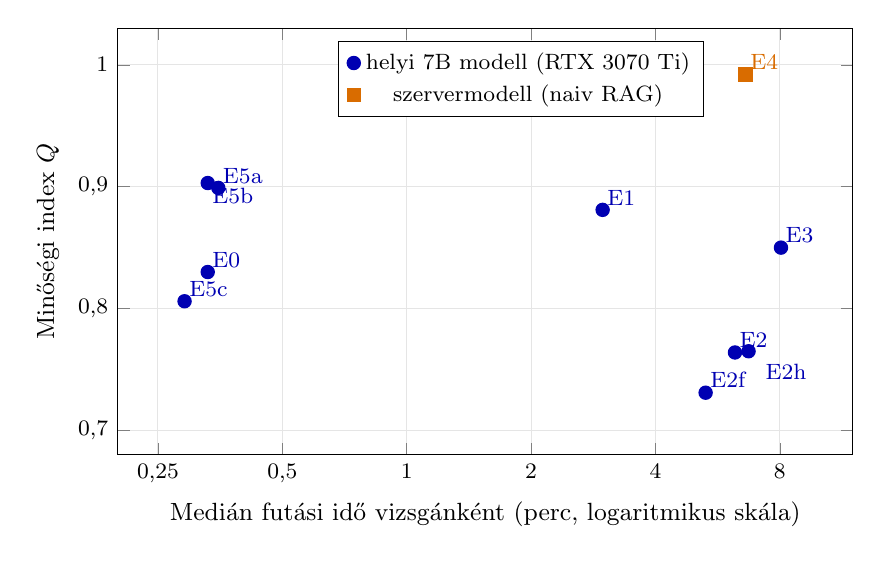
\begin{tikzpicture}
\begin{axis}[
  width=0.9\textwidth, height=7cm, xmode=log,
  xmin=0.2, xmax=12, ymin=0.68, ymax=1.03,
  xtick={0.25,0.5,1,2,4,8}, xticklabels={{0,25},{0,5},1,2,4,8},
  yticklabel style={/pgf/number format/.cd, fixed, precision=2, use comma},
  xlabel={Medián futási idő vizsgánként (perc, logaritmikus skála)}, ylabel={Minőségi index $Q$},
  xlabel style={font=\small}, ylabel style={font=\small},
  tick label style={font=\footnotesize}, grid=major, grid style={gray!20},
  nodes near coords, point meta=explicit symbolic,
  every node near coord/.style={font=\footnotesize, anchor=south west, inner sep=1.5pt},
  legend style={font=\footnotesize, at={(0.30,0.97)}, anchor=north west}]
\addplot[only marks, mark=*, mark size=2.4pt, blue!70!black] coordinates {
  (0.33,0.830) [E0] (2.98,0.881) [E1] (6.23,0.764) [E2] (5.29,0.731) [E2f]
  (6.72,0.765) [] (8.05,0.850) [E3] (0.35,0.899) [E5a] (0.29,0.806) [E5c]};
\addlegendentry{helyi 7B modell (RTX 3070 Ti)}
\addplot[only marks, mark=square*, mark size=2.4pt, orange!85!black] coordinates {(6.61,0.992) [E4]};
\addlegendentry{szervermodell (naiv RAG)}
\node[font=\footnotesize, anchor=west, blue!70!black] at (axis cs:7.0,0.748) {E2h};
\addplot[only marks, mark=*, mark size=2.4pt, blue!70!black, forget plot, every node near coord/.style={font=\footnotesize, anchor=north west, inner sep=1.5pt}] coordinates {(0.33,0.903) [E5b]};
\end{axis}
\end{tikzpicture}
\caption{Minőség és futási idő a pilotban. A tervezett karok egy nagyságrenddel lassabbak; a
minőségnövekedést csak a tervezés (\arm{E1}) hozta meg ellenőrzés nélkül.}
\label{fig:minoseg-ido}
\end{figure}

Az ellenőrző karok hívásszáma (59--101) messze meghaladja \az{\eqref{eq:callbounds}} szerinti alsó korlátot
(21--31), ami azt jelzi, hogy a kérdések jelentős része legalább egyszer elbukott. Az \arm{E2} kar
slotonként átlagosan 3,1 generálást igényelt; \az{\eqref{eq:expattempts}} képletet a tartalékfogalommal együtt
alkalmazva ez $p\approx0{,}3$ körüli kísérletenkénti átmenési valószínűségnek felel meg -- azaz a kis
modell ellenőrzője a kérdések kétharmadát első körben elutasította, miközben (az előző szakasz
szerint) ítélete a bíróéval nem egyezett. Az ellenőrzés tehát a pilotban a hívásszámot 60--100-szorosára
növelte anélkül, hogy információt adott volna. A tervezés (\arm{E1}) ezzel szemben 23 hívással mérhető
minőségjavulást hozott; a pilot alapján a fő vizsgálatban a tervezés bizonyítása, az ellenőrzés
pedig érdemének igazolása a feladat.

\section{Darabolási stratégiák}

Az egyhívásos alapvonalat három darabolási változattal is összevetettük (\ref{tab:pilot-fo}. és \ref{tab:hosszak}.~táblázat). A
rögzített, 800 karakteres ablakok (\arm{E5c}) adták a leggyengébb eredményt: a kérdéspárok 45\,\%-a
közel-duplikátum volt (a szemantikus darabolásnál 10--16\,\%), és a bíró disztraktorpontszáma 3,0-ra
esett (a szemantikus változatoknál 3,5--3,9). A szórásalapú küszöb (\arm{E5b}) és a régi kódoló
(\arm{E5a}) 0,90-es indexet ért el. Az utóbbi eredmény nem jelenti a régi kódoló előnyét: egy
512 tokennél rövidebb dokumentumon a régi és az új kódoló \emph{azonos} darabokat ad, így az \arm{E0}
és az \arm{E5a} közötti különbség kizárólag a futásról futásra jelentkező zajból ered.


\section{Futásról futásra jelentkező zaj}
\label{sec:zaj}

Az \arm{E0} és az \arm{E5a} kar a pilotban azonos darabokat, azonos visszakeresett kontextust és azonos
magokat kapott (ezt a nyers adatok, a \code{exams.jsonl} fájlok \code{retrieved} mezői igazolják),
mégis eltérő kérdéseket, és 0,83, illetve 0,90 minőségi indexet adtak. Ez a különbség tehát egy
természetes kontrollkísérlet: a teljes mérési láncot változatlanul hagyva, csak az ismétlés miatt
0,07-es eltérés adódott. Az ok az, hogy a GPU-n végzett következtetés alacsony hőmérsékleten és rögzített
maggal sem bitre reprodukálható (a párhuzamos lebegőpontos redukciók sorrendje nem determinisztikus).

Ebből két következtetés adódik. \emph{Egyrészt}, egyetlen dokumentumon a 0,07-nél kisebb különbségek
zajnak tekintendők -- a pilot szinte minden helyi karpárjának különbsége ebbe a sávba esik, a tervezés
hatása ($+0{,}05$) is. \emph{Másrészt}, a zaj csökkentésének hatékony módja nem a magok számának
növelése egyetlen dokumentumon, hanem a dokumentumok számának növelése, mert a fő vizsgálat
hipotézisei dokumentumok populációjára vonatkoznak. A fő vizsgálat ezért 39 dokumentumon,
dokumentumszintű statisztikával fut.

\section{Példák}

\Az{\ref{tab:peldak}}.~táblázat négy pilotkérdést mutat eredeti, magyar nyelvükön, a bíró ítéletével. A
példák a fenti eredmények tipikus eseteit illusztrálják: a naiv alapvonal téves kulcsát, a tervezett
kar alá nem támasztott részletét, a szivárgó kérdést és a szervermodell jó kérdését.

\begin{table}[htbp]
\centering
\caption{Pilotkérdések eredeti nyelven (* = megjelölt kulcs), a bíró ítéletével.}
\label{tab:peldak}
\footnotesize
\begin{tabularx}{\textwidth}{@{}>{\raggedright\arraybackslash}p{1.2cm}>{\raggedright\arraybackslash}X@{}}
\toprule
\arm{E0} & \emph{A kávé felfedezéséhez milyen században jutott el a velencei kereskedők révén?}
9.~század* / 10.~század / 8.~század / 11.~század. \textbf{Bíró:} nem alátámasztott -- a forrás szerint a
kávé a 17.~században jutott el Velencébe; a 9.~század az etióp legenda ideje. Egyik opció sem helyes;
helyesség 1/5. \\
\midrule
\arm{E1} & \emph{A pörkölés hőmérsékeltségének milyen hatással van az italt és a koffeintartalomra?}
Kulcs: \emph{A sötét pörkölés testesebb, füstösebb és keserűbb ízvilágot eredményez, de a
koffeintartalom csökken.}* \textbf{Bíró:} az ízhatást a forrás igazolja, a koffeintartalomról azonban nem
szól, így a kulcs nem alátámasztott; a disztraktorok jók; helyesség 1/5. (A törzs nyelvtani hibája a 7B
modell magyar nyelvi korlátját is mutatja.) \\
\midrule
\arm{E3} & \emph{„A kávéfogyasztás szokása Etiópiából hamar átterjedt a szomszédos Jemenbe, majd az arab
világba, Európába pedig a 17.~században jutott el a velencei kereskedők révén.”} Kulcs: ugyanez a
mondat*; disztraktorok: a mondat a 16., 18., illetve 15.~századdal. \textbf{Bíró:} alátámasztott, vakon
helyes, helyesség 5/5 -- noha a „törzs” nem kérdés, és a választ szó szerint tartalmazza. \\
\midrule
\arm{E4} & \emph{Mennyit tesz ki az Arabica a globális kávétermelésből?} Mintegy 70 százalékát* /
Mintegy 30 százalékát / Mintegy 50 százalékát / Mintegy 90 százalékát. \textbf{Bíró:} a forrás a 70\,\%-ot
közvetlenül kimondja; a többi arány hihető, de a szöveg cáfolja; helyesség 5/5. \\
\bottomrule
\end{tabularx}
\end{table}

\section{A hipotézisek előzetes értékelése}

\Az{\ref{tab:hipotezisek}}.~táblázat összefoglalja, hogy a pilot milyen irányú bizonyítékot szolgáltat az
egyes hipotézisekhez. Hangsúlyozzuk, hogy ezek egyetlen dokumentumon, szignifikanciavizsgálat nélkül
tett, leíró megfigyelések; a hipotézisek eldöntése a fő vizsgálat feladata.

\begin{table}[htbp]
\centering
\caption{A hipotézisek és a pilot által szolgáltatott előzetes, leíró bizonyíték.}
\label{tab:hipotezisek}
\small
\begin{tabularx}{\textwidth}{@{}>{\raggedright\arraybackslash}p{2.6cm}>{\raggedright\arraybackslash}X>{\raggedright\arraybackslash}p{2.6cm}@{}}
\toprule
Hipotézis & Pilot megfigyelés & Irány \\
\midrule
\ref{h:terv}.\ Tervezés & alátámasztottság $+6$, lefedettség $+8$ pp, forma változatlan; a különbség a zajsávon belül & támogató, nem döntő \\
\ref{h:verif}.\ Ellenőrzés & alátámasztottság változatlan, vak megoldhatóság $-16$ pp; $\kappa\in[-0{,}14;0{,}07]$ & ellentmondó (önellenőrzésre) \\
\ref{h:lefed}.\ Lefedettség & a szervermodell naiv RAG-gal 25\,\% lefedettséget ért el; a \arm{B-doc} kar még nem futott & támogató (közvetett) \\
\ref{h:helyi}.\ Helyi vs.\ szerver & különbség 0,09--0,11; memória 5,4--5,9\,GiB & részben támogató \\
\ref{h:meres}.\ Mérés & oktatói értékelés még nincs; a bíró a szivárgó kérdéseket nem büntette & nyitott; kockázat azonosítva \\
\bottomrule
\end{tabularx}
\end{table}

\section{A fő vizsgálat eredményei}
\label{sec:fo-vizsgalat}

A fő vizsgálat (\code{eval-v1}, 39 dokumentum, \az{\ref{tab:karok}}.~táblázat összes kara, oktatói
értékeléssel) futása e dolgozat lezárásakor folyamatban van. Eredményei a keretrendszer
\code{report} lépésével, a pilottal azonos formában, automatikusan kerülnek \az{\ref{tab:fo-vizsgalat}}.~táblázatba és a hozzá tartozó szignifikanciatáblába. A táblázat szerkezetét
itt rögzítjük; a piros mezők a fő futás adataira várnak.

\begin{table}[htbp]
\centering
\caption{A fő vizsgálat eredményei (39 dokumentum; átlag és 95\,\%-os bootstrap-CI; páros
Wilcoxon-próba Holm-korrekcióval a referenciakarhoz képest). \tbd{A fő futás után kitöltendő.}}
\label{tab:fo-vizsgalat}
\small
\begin{tabular}{@{}llccccc@{}}
\toprule
Kar & Ref. & $Q$ [95\,\% CI] & Alát. & Lef. & $\tilde p$ (Holm) & $r_{rb}$ \\
\midrule
\arm{B-doc-L} & -- & \tbd{--} & \tbd{--} & \tbd{--} & -- & -- \\
\arm{E0}  & -- & \tbd{--} & \tbd{--} & \tbd{--} & -- & -- \\
\arm{E1}  & \arm{E0} & \tbd{--} & \tbd{--} & \tbd{--} & \tbd{--} & \tbd{--} \\
\arm{E2}  & \arm{E1} & \tbd{--} & \tbd{--} & \tbd{--} & \tbd{--} & \tbd{--} \\
\arm{E2x} & \arm{E2} & \tbd{--} & \tbd{--} & \tbd{--} & \tbd{--} & \tbd{--} \\
\arm{E3}  & \arm{E2} & \tbd{--} & \tbd{--} & \tbd{--} & \tbd{--} & \tbd{--} \\
\arm{E4}  & \arm{E0} & \tbd{--} & \tbd{--} & \tbd{--} & \tbd{--} & \tbd{--} \\
\arm{E4b} & \arm{E2} & \tbd{--} & \tbd{--} & \tbd{--} & \tbd{--} & \tbd{--} \\
\arm{B-doc-S} & -- & \tbd{--} & \tbd{--} & \tbd{--} & -- & -- \\
\bottomrule
\end{tabular}
\end{table}
